\documentclass[11pt]{article}
\usepackage{hyperref} 
\usepackage{amsmath, amsfonts, amssymb}
\usepackage{graphicx}
\usepackage{float}
\usepackage[margin=1in]{geometry}

\parindent0px

\emergencystretch=0pt
\pretolerance=150
\tolerance=10000
\hbadness=10000
\hfuzz=0pt

\title{Probability and Statistics by DeGroot Notes}
\author{Nathan Ueda}
\date{\today} 

\begin{document}
\maketitle 
\pagebreak
\tableofcontents 
\pagebreak

\section{Introduction to Probability}
\subsection{The History of Probability}
The use of probability to measure uncertainty and variability dates back hundredes of years.

\subsection{Interpretations of Probability}

\textbf{Probability Interpretations}
\begin{itemize}
    \item Frequency: If an experiment is carried out many times, the frequency with which a
    particular outcome occurred would define its probability.
    \item Classical: If an outcome of some experiment must be one of $n$ different, equally
    likely outcomes, the probability of each outcome is $\frac{1}{n}$.
    \item Subjective: An entity assigns probabilities to each possible outcome.
\end{itemize}

Probability theory does not depend on intepretation.

\subsection{Experiments and Events}

Probability allows us to quantify how likely an outcome is to occur. \\

\textbf{Experiments:} Any process in which the possible outcomes can be identified ahead of time.
\textbf{Events:} A well defined set of possible outcomes of the experiment (such as rolling an 
even number on a fair dice). \\

Although there is controversy in regard to the proper meaning and interpration of some of the
probabilities that are assigned to the outcomes of many experiements, once these probabilities
are assigned, there is complete agreemenet upon the mathematical theory of probability. \\

Almost all work in the mathematical theory of probability is related to:
\begin{itemize}
    \item Methods for determining probabilities of certain events from given probabilities for
    each possible outcome in an experiment.
    \item Methods for revising probabilities of events when additional relevant information is 
    obtained.
\end{itemize}

\subsection{Set Theory}

\textbf{Sample Space:} The collection of all possible outcomes of an experiment. \\
\textbf{Empty Set:} Subset of $S$ containing no elements, denoted $\emptyset$, representing
any events that cannot occur. \\
\textbf{Complement:} For some set $A$, its complement, denoted $A^c$, is the set containing all 
elements of $S$ not in $A$. \\
\textbf{Union:} For $n$ sets $A_1, \ldots, A_n$, their union, denoted $A_1 \cup \ldots \cup A_n
$ or $ \bigcup_{i=1}^{n} A_i $, is defined as the set containing all outcomes that belong to at
least one of these $n$ sets. \\
\textbf{Intersection:} For $n$ sets $A_1, \ldots, A_n$, their intersection, denoted $A_1 \cap 
\ldots \cap A_n $ or $ \bigcap_{i=1}^{n} A_i $, is defined as the set containing the elements 
common to all these $n$ sets. \\
\textbf{Disjoint/Mutually Exclusive:} Two sets $A$ and $B$ are disjoint/mutually exclusive if 
they have no outcomes in common, that is, if $ A \cap B = \emptyset $, representing that both
$A$ and $B$ cannot occur.

\subsection{The Definition of Probability}

Axioms of Probability:
\begin{enumerate}
    \item For every event $A$, $P(A) \ge 0$.
    \item $P(S) = 1$.
    \item $P( \bigcup_{i=1}^{\infty} A_i) = \sum_{i=1}^{\infty}P(A_i)$.
\end{enumerate}

Basic Theorems:
\begin{enumerate}
    \item $P(\emptyset) = 0$.
    \item For every finite sequence of $n$ disjoint events, $A_1, \ldots, A_n$, $P( 
    \bigcup_{i=1}^{n} A_i) = \sum_{i=1}^{n}P(A_i)$.
    \item For every event $A$, $P(A^c) = 1 - P(A)$.
    \item If $A \subset B$, then $P(A) \le P(B)$.
    \item For every event $A$, $0 \le P(A) \le 1$.
    \item For every two events $A$ and $B$, $P(A \cap B^c) = P(A) - P(A \cap B)$.
    \item For every two events $A$ and $B$, $P(A \cup B) = P(A) + P(B) - P(A \cap B)$.
    \item Bonferroni Inequality: For all events $A_1, \ldots, A_n$, $P(\bigcap_{i=1}^{n} A_i) 
    \ge 1 - \sum_{i=1}^{n} P(A_i^c)$.
\end{enumerate}

\subsection{Finite Sample Spaces}

Simple Sample Space
\begin{itemize}
    \item Has a finite number ($n$) of possible outcomes.
    \item Each outcome has an equal probability ($\frac{1}{n}$).
    \item If an event $A$ has $m$ outcomes, then $P(A) = \frac{m}{n}$.
\end{itemize}

\subsection{Counting Methods}

\textbf{Multiplication Rule:} An experiment with $k$ parts where the $i$th part has $n_i$ 
possible outcomes (regardless of which specific outcomes have occurred in the other parts) has 
a sample space $S = n_1 n_2 \ldots n_k$. \\

\textbf{Permutations ($P_{n,k}$):}
\begin{itemize}
    \item Number of ways to arrange a set (order matters).
    \item Sampling considering $n$ different items and making $k$ choices from them.
    \begin{itemize}
        \item Sampling with replacement: $n^k$.
        \item Sampling without replacement: $n(n-1) \ldots (n-k+1)$.
        \begin{itemize}
            \item $n$ options for first choice, $n-1$ options for second choice, $n-k+1$ 
            options for $k$th choice.
        \end{itemize}
    \end{itemize}
    
    \item The number of permutations of $n$ different items is $P_{n,n} = n$!.
    \item The number of permutations of $n$ different items making $k$ choices ($0 \le k \le 
    n$) is
        \[P_{n,k} = n(n-1) \ldots (n-k+1)\]
        \[P_{n,k} = n(n-1) \ldots (n-k+1) \left(\frac{1}{1}\right)\]
        \[P_{n,k} = n(n-1) \ldots (n-k+1) \left(\frac{(n-k)(n-k-1) \ldots 1}{(n-k)(n-k-1) 
        \ldots 1}\right)\]
        \[P_{n,k} = \frac{n(n-1) \ldots (n-k+1)(n-k)(n-k-1) \ldots 1}{(n-k)(n-k-1) \ldots 1}\]
        \[P_{n,k} = \frac{n!}{(n-k)!}\]
\end{itemize}

\subsection{Combinatorial Methods}
\textbf{Combinations ($C_{n,k}$):}
\begin{itemize}
    \item Number of subsets (order does not matter).
    \item Permutations may be thought of as combinations of size $k$ chosen out of $n$, 
    multiplied by the number of ways to arrange the size $k$ subsets, $k$!. More formally, this
    says 
    \[ P_{n,k} = C_{n,k} k!\]
    \item Combinations (binomial coefficient) are the number of distinct subsets of size $k$ 
    that can be chosen from a set of size $n$ (this is the same formula as for permutations,
    except we are dividing out the number of ways we can rearrange the subsets, $k$!, since 
    order does not matter): 
        \[C_{n,k} = {n \choose k} = \frac{P_{n,k}}{k!} = \frac{\frac{n!}{(n-k)!}}{k!} =  \frac{n!}{(n-k)!k!} \]
    \item Combinations without replacement: ${n+k-1 \choose k}$.
\end{itemize}

\subsection{Multinomial Coefficients}

The total number of different ways of dividing $n$ elements into $k$ groups is 
\[ {n \choose n_1, n_2, \ldots, n_k} = {n \choose n_1} {n - n_1 \choose n_2} {n - n_1 - n_2 
\choose n_3} \cdots {n - n_1 - \cdots - n_{k-2} \choose n_{k-1}} = \frac{n!}{n_1!n_2! \cdots 
n_k!}\]

\subsection{The Probability of a Union of Events}

\begin{itemize}
    \item Union of two events $A_1$ and $A_2$: \[P(A_1 \cup A_2) = P(A_1) + P(A_2) - P(A_1 \cap
    A_2)\]
    \item Union of three events $A_1$, $A_2$, and $A_3$: \[P(A_1 \cup A_2 \cup A_3) = P(A_1) + 
    P(A_2) + P(A_3) - \left[ P(A_1 \cap A_2) + P(A_1 \cap A_3) + P(A_2 \cap A_3) \right] \] \[ 
    + P(A_1 \cap A_2 \cap A_3)\]
    \item Union of $n$ events $A_1, \ldots, A_n$: \[ P \left(\bigcup_{i=1}^{n} A_i\right) = 
    \sum_{i=1}^{n} P(A_i) - \sum_{i<j}P(A_i \cap A_j) + \sum_{i<j<k}P(A_i \cap A_j \cap A_k) -
    \] \[ \sum_{i<j<k<l} P(A_i \cap A_j \cap A_k \cap A_l) + \cdots + {(-1)}^{n+1} P(A_1 \cap 
    A_2 \cap \cdots \cap A_n)\]
\end{itemize}

\section{Conditional Probability}

\subsection{The Definition of Conditional Probability}

\begin{itemize}
    \item Conditional probability is the updating of probabilities when certain events are
    observed.
    \item The updated probability of event $A$ after we learn that event $B$ has occured is the
    conditional probability of $A$ given $B$, denoted $P(A|B)$.
    \item When we go from $P(A)$ to $P(A|B)$, we say we are conditioning on $B$.
    \item For $P(B) > 0$ \[P(A|B) = \frac{P(A \cap B)}{P(B)}\].
    \item Intuitively, this is saying the probability of $A$ occurring, given $B$ has occurred
    is equal to the outcomes where both $A$ and $B$ occurred (which makes sense since we know 
    $B$ has occurred and we want to find the probability of $A$ also occurring) divided by the 
    probability of $B$ occurring (which makes sense since we know $B$ occurred, we can 
    renormalize the sample space to only contain outcomes where $B$ occurred).
\end{itemize}

\textbf{Multiplication Rule for Conditional Probabilities}
\begin{itemize}
    \item For 2 events $A,B$
    \begin{itemize}
        \item If $P(B) > 0$ \[P(A \cap B) = P(B)P(A|B)\]
        \item If $P(A) > 0$ \[P(A \cap B) = P(A)P(B|A)\]
    \end{itemize}
    \item For $n$ events $A_1, \ldots, A_n$ such that $P(A_1 \cap \ldots \cap A_{n-1}) > 0$ 
    \[P(A_1 \cap \ldots \cap A_n) = P(A_1)P(A_2|A_1)P(A_3|A_1 \cap A_2) \ldots P(A_n|A_1 \cap
    \ldots A_{n-1})\]
    \item For $n$ events $A_1, \ldots, A_n, B$ such that $P(B) > 0$ and $P(A_1 \cap \ldots \cap
    A_{n-1}) > 0$ 
    \[P(A_1 \cap \ldots \cap A_n|B) = P(A_1|B)P(A_2|A_1 \cap B)P(A_3|A_1 \cap A_2 \cap B) 
    \ldots P(A_n|A_1 \cap \ldots A_{n-1} \cap B)\]
\end{itemize}

\textbf{Law of Total Probability}
\begin{itemize}
    \item Tells us that to get the unconditional probability of $A$, we can divide the sample
    space into disjoint slices $B_j$, find the conditional probability of $A$ within each of 
    these slices, then take a weighted sum of the conditional probabilities, where the weights
    are the probabilities $P(B_j)$.
    \item Often used in tandum with Bayes' Rule.
    \item Relates conditional probability to unconditional probability .
    \item Partition: Let $S$ denote the sample space and consider $k$ events $B_1, \ldots, B_k$
    in $S$ such that $B_1, \ldots, B_k$ are disjoint and $\bigcup_{i=1}^{k}B_i = S$. Then 
    events $B_1, \ldots, B_k$ form a partition in $S$. In other words, only one of these events
    can occur and combined they fill the entire sample space.
    \item Suppose events $B_1, \ldots, B_k$ form a partition of the space $S$ and $P(B_j) > 0$
    for $j = 1, \ldots, k$. Then \[P(A) = \sum_{j=1}^{k} P(B_j \cap A) = \sum_{j=1}^{k} P(B_j)
    P(A|B_j)\].
    \item Conditional LOTP \[P(A|C)= \sum_{j=1}^{k}P(B_j|C)P(A|B_j \cap C)\].
\end{itemize}

\subsection{Independent Events}

\textbf{Independence of 2 Events:}
\begin{itemize}
    \item Two events are independent if learning that one occurred does not change the
    probability of the other event.
    \item Two events $A$ and $B$ with positive probabilities are independent if 
    \[P(A \cap B) = P(A)P(B)\] 
    \item Similarly, two events $A$ and $B$ with positive probabilities are independent if 
    \[P(A|B) = P(A) \text{ and } P(B|A)=P(B)\]
    \item If two events $A$ and $B$ are independent, then $A$ and $B^C$ are independent
\end{itemize}

\textbf{Independence of k Events:}
\begin{itemize}
    \item For $k$ events, if knowing what happened with any particular subset of the events 
    gives us no information about what happened with the events not in the subset, the events
    are independent.
    \item $k$ events are (mutually) independent if 
    \begin{itemize}
        \item Any pair $P(A_i \cap A_j) = P(A_i)P(A_j) \text{ for } i \ne j$ 
        \item Any triplet $P(A_i \cap A_j \cap A_k) = P(A_i)P(A_j)P(A_k) \text{ for } i \ne j 
        \ne k$
        \item $\ldots$
        \item The n-tuplet $P(A_1 \cap \ldots \cap A_n) = P(A_1) \ldots P(A_n) $
    \end{itemize}
\end{itemize}

When deciding whether or not to model events as independent, try to answer the following 
question: ``If I were to learn that some of these events occurred, would I change the 
probabilities of any of the others?'' \\

\textbf{Conditional Independence:}
\begin{itemize}
    \item Two events $A$ and $B$ are conditionally independent given $E$ if $P(A \cap B|E) =
    P(A|E)P(B|E)$.
    \item It is defined as independence but with respect to the conditional probabilities.
\end{itemize}

\subsection{Bayes' Theorem}

\begin{itemize}
    \item Bayes' Theorem relates $P(A|B)$ to $P(B|A)$.
    \item This is important as often it is easier to solve either $P(A|B)$ or $P(B|A)$.
    \item Suppose that we are interested in which of several disjoint events $A_1, \ldots, A_k$
    will occur and that we will get to observe some other event $B$. If $P(B|A_i)$ is available
    for each $i$, then Bayes' theorem is a useful formula for computing the conditional 
    probabilities of the $A_i$ events given $B$, that is, $P(A_i|B)$ for each $i$.
\end{itemize}


\textbf{Bayes' Theorem for 2 Events}
\begin{itemize}
    \item \[P(A|B) = \frac{P(B|A)P(A)}{P(B)}\]
    \item It is often common to use LOTP in the denominator
    \[P(A|B) = \frac{P(B|A)P(A)}{\sum_{i=1}^{n}P(B|A_i)P(A_i)} = 
    \frac{P(B|A)P(A)}{P(B|A)P(A) + P(B|A^c)P(A^c)} \]
\end{itemize}



\textbf{Bayes' Theorem for $n$ Events}

\[P(A_i|B)=\frac{P(B|A_i)P(A_i)}{\sum_{j=1}^{n}P(B|A_j)P(A_j)}\]

\textbf{Prior vs. Posterior Probabilities}
\begin{itemize}
    \item Prior probabilities represent probabilities \textit{before} new evidence is 
    introduced.
    \begin{itemize}
        \item $P(A)$
    \end{itemize}
    \item Posteror probabilities represent probabilities \textit{after} the new evidence in 
    taken into consideration.
    \begin{itemize}
        \item $P(A|B)$
    \end{itemize}
\end{itemize}

\textbf{Conditional Version of Bayes' Theorem}
\[P(A_i|B \cap C) = \frac{P(B|A_i \cap C)P(A_i|C)}{\sum_{j=1}^{n}P(B|A_j \cap C)P(A_j|C)}\]

\subsection{The Gambler's Ruin Problem}

\textbf{High Level Problem Overview:} Consider two gamblers with finite resources who 
repeatedly play the same game against each other. Using the tools of conditional probability, 
we can calculate the probability that each of the gamblers will eventually lose all of his 
money to the opponent. As this game ends only when one of the gamblers has no money left, this
problem is fittingly called, the Gambler's Ruin problem. \\

\textbf{Problem Statement}
\begin{itemize}
    \item Two gamblers, $A$ and $B$, make \$1 bets each round.
    \item $A$ has a probability $p$ of winning, $B$ has probability $1-p$ of winning.
    \item $A$ starts with $k$ dollars, $B$ starts with $k-i$ dollars, for a combined fortune of
    $k$.
    \item The game continues until one of the gamblers has 0 dollars left.
    \item The goal is to determine the probability that $A$ will reach $k$ dollars before 0.
\end{itemize}

\section{Random Variables and Distributions}
\subsection{Random Variables and Discrete Distributions}

\textbf{Random Variables}
\begin{itemize}
    \item A function that maps each outcome in the sample space to the real line.
    \item Two main types of random variables: discrete and continuous random variables.
    \item Main tool used for modeling unknown quantities in statistical analysis.
\end{itemize}

\textbf{Distributions}
\begin{itemize}
    \item A distribution specifies the probabilities of all events associated with a random
    variable (maps outcomes to probabilities).
\end{itemize}

\textbf{Discrete Distributions}
\begin{itemize}
    \item Distributions that assign positive probability to at most countably many different
    values.
    \item Discrete distributions can be characterized by its probability function (p.f.) aka
    probability mass function (p.m.f).
\end{itemize}

\textbf{Discrete Random Variables}
\begin{itemize}
    \item A random variable with a discrete distribution.
    \item Is a discrete r.v. if the r.v. can take only a finite number $k$ of different values
    $x_1, \ldots x_k$ or, at most, an infinite sequence of different values $x_1, x_2, \ldots $
\end{itemize}

\textbf{Probability Function}
\begin{itemize}
    \item A function that describes the probabilities of different values of a r.v.
    \item For a discrete r.v., the p.f. of $X$ is defined as the function $f$ such that for 
    every real number $x$, \[f(x)=P(X=x)\]
    \item If $x$ is not a possible value of $X$, then $f(x)=P(X=x)=0$
    \item The support of $X$ is all values $x$ such that $f(x)=P(X=x)>0$.
    \item To be a valid p.f.
    \begin{itemize}
        \item The probabilities of all possible outcomes of $X$ sum to 1. More formally, if the
        sequence $x_1, x_2, \ldots$ includes all the possible values of $X$, then $\sum_{i=1}^
        {\infty} f(x_i) = 1$.
        \item All possible values of $X$ have a probability greater than 0 and all other values 
        have a probability of 0.
    \end{itemize}
    \item A p.f. is only for discrete distributions.
\end{itemize}

\textbf{Example}
    \begin{itemize}
        \item In an experiment in which a fair coin is tossed 2 times, we can define a random 
        variable $X$ to represent the number of heads in each outcome.
        \item The possible outcomes in the sample space are $S = \{TT, HT, TH, HH\}$.
        \item $X(TT)=0,\ X(TH)=1,\  X(HT)=1,\ X(HH)=2$.
        \item Therefore, the p.f. of $X$ is the function $f$ given by 
        \begin{itemize}
            \item $f(0) = P(X=0) = 1/4 $
            \item $f(1) = P(X=1) = 1/2 $
            \item $f(2) = P(X=2) = 1/4 $
        \end{itemize}
    \end{itemize} 

\textbf{Common Named Distributions}
\begin{itemize}
    \item Some random variables has distributions that occur so frequently they are given 
    names. 
    \item These common named distributions represent a family of distributions (for example, 
    there are a family of Bernoulli distributions, not just one). What allows us to determine 
    the specific distribution we have (the specific Bernoulli distribution we have), are 
    parameters (for Bernoulli, this is the value for $p$)
\end{itemize}

\textbf{Bernoulli Distributions}
\begin{itemize}
    \item A distribution of the probabilities of a single experiment asking a yes-no question.
    \item A r.v. $X$ that takes on only two values 1 and 0 (success and failure).
    \item Has one parameter, $p$.
    \item Written $X \sim \text{Bern}(p)$.
    \item p.f. of $X$
    \[ P(X=x) = f(x) = \begin{cases} 
        p & \text{for } x=1 \\
        1-p & \text{for } x=0 \\
        0 & \text{otherwise}
     \end{cases}
  \]
\end{itemize}

\textbf{Discrete Uniform Distributions}
\begin{itemize}
    \item A distribution where each outcome for the r.v. has an equally likely probability.
    \item A r.v. $X$ where, for 2 integers $a,b$ where $a \le b$, the value of $X$ is equally 
    likely to be each of the integers $a, \ldots, b$.
    \item A uniform distribution on a set of $k$ integers has probability of $1/k$ on each 
    integer.
    \item Has two parameters, $a,b$.
    \item Written $X \sim \text{DUnif}(a,b)$.
    \item p.f. of $X$
    \[ P(X=x) = f(x) = \begin{cases} 
        \frac{1}{b-a+1} & \text{for } x=a, \ldots, b \\
        0 & \text{otherwise}
     \end{cases}
  \]
\end{itemize}

\textbf{Binomial Distributions}
\begin{itemize}
    \item A distribution that is based upon a r.v. denoting the number of successes in $n$ 
    independent Bernoulli trials (an experiment that can end only in success or failure).
    \item Suppose that $n$ independent Bernoulli trials  are performed, each with success 
    probability $p$. If we let $X$ be the number of success, then the distribution of $X$ is 
    called the Binomial distribution with parameters $n$ and $p$. 
    \item Has two parameters, $n, p$.
    \item Written $X \sim \text{Bin}(n,p)$.
    \item p.f. of $X$
    \[ P(X=x) = f(x) = \begin{cases} 
        {n \choose x}p^x{(1-p)}^{n-x} & \text{for } x=0, \ldots, n \\
        0 & \text{otherwise}
     \end{cases}
  \]
  \begin{itemize}
    \item The probability of obtaining exactly $x$ successes and $n-x$ failures is $p^x{(1-p)}
    ^{n-x}$. Since there are ${n \choose x}$ ways of ordering this, its follows that $P(X=x)=
    {n \choose x}p^x{(1-p)}^{n-x}$.
  \end{itemize}
  \item The Bernoulli distribution is just a special case of the Binomial distribution where 
  $n=1$, that is, Bin$(1, p)$.
\end{itemize}

\subsection{Continuous Distributions}

\textbf{Continuous Distributions}
\begin{itemize}
    \item Distributions that have a range of values that are uncountably infinite. 
    \item Continuous distributions can be characterized by its probability density function 
    (p.d.f.)
    \item Assign probability 0 to individual values, that is, $P(X=x)=0$ for every number $x$.
\end{itemize}

\textbf{Continuous Random Variables}
\begin{itemize}
    \item A random variable with a continuous distribution.
\end{itemize}

\textbf{Probability Density Function}
\begin{itemize}
    \item A nonnegative function $f$ for a r.v. $X$ such that the integral of $f$ over each 
    interval $[a,b]$ gives the probability that $X$ is in the interval, that is, $P(a \le X 
    \le b) = \int_{a}^{b} f(x) \,dx$.
    \item Similarly, $P(X \ge a) = \int_{a}^{\infty} f(x) \,dx$ and $P(X \le b) = \int_
    {-\infty}^{b} f(x) \,dx$.
    \item Density is not probability (density can be greater than 1). The p.d.f. of $X$, 
    $f(x)$, itself is not the probability that $X$ is near $x$, instead, the integral of $f$ 
    over values near x gives the probability that $X$ is near $x$, and the integral is never 
    greater than 1.
    \item Since the endpoints have probability 0, for an interval $(a,b)$, $P(a < X < b) = 
    P(a \le X \le b) = P(a < X \le b) =  P(a \le X < b)$
    \item The support of $X$ is all values $x$ such that $f(x)=P(X=x)>0$.
    \item To be a valid p.d.f.
    \begin{itemize}
        \item The p.d.f. of $X$ must integrate to 1, that is, $\int_{-\infty}^{\infty} f(x) \,dx=1$.
        \item For all $x$, $f(x) \ge 0$.
    \end{itemize}
    \item To get a desired probability, integrate the p.d.f. over the appropriate range.
    \item In general, we can think of $f(x) \,dx$ as the probability of $X$ being in an 
    infinitesimally small interval containing $x$, of length $\,dx$,
\end{itemize}

\textbf{Uniform Distributions}
\begin{itemize}
    \item A Uniform r.v. on the interval $(a,b)$ is a completely random number, which speicifies 
    that the p.d.f. is constant over the interval.
    \item Has two parameters, $a,b$.
    \item Written $X \sim \text{Unif}(a,b)$.
    \item p.d.f. of $X$
    \[ f(x) = \begin{cases} 
        \frac{1}{b-a} & \text{for } a \le x \le b \\
        0 & \text{otherwise}
     \end{cases}
  \]
\end{itemize}

\textbf{Normalizing Constants}
\begin{itemize}
    \item Often, we will have a p.d.f without a specified value for $c$, 
    the normalizing constant. 
    \item This happens especially often when we find sampling distributions 
    of summaries of observed data where we can determine the p.d.f of a 
    r.v. except for the constant factor.
    \item The constant is unique.
    \item Using the fact that the p.d.f must integrate to 1, we can solve 
    for $c$.
    \item Example:
    \[\int_{0}^{4}cx \,dx = 1\]
    \[c\int_{0}^{4}x \,dx = 1\]
    \[c\frac{x^2}{2}\rvert_0^4 = 1\]
    \[c\left(\frac{4^2}{2}-0\right)= 1\]
    \[c\left(\frac{16}{2}\right)= 1\]
    \[8c= 1\]
    \[c= \frac{1}{8}\]
\end{itemize}

\subsection{The Cumulative Distribution Function}   

\textbf{Cumulative Distribution Function}
\begin{itemize}
    \item A function of a r.v. $X$, denoted $F$, that gives the probability that the r.v. is 
    less than or equal to $x$ \[F(x)=P(X \le x) \text{ for } -\infty < x < \infty\]
    \item While a p.f is defined only for discrete r.v.s and a p.d.f is defined for only 
    continuous r.v.s, a c.d.f. is defined for both discrete and continuous r.v.'s.
    \item The c.d.f. is another way of characterizing the distribution of a r.v.
    \item The value of $F$ at every point $x$ must be a number $F(x)$ in the interval $[0,1]$
    because $F(x)$ is the probability of the event ${X \le x}$.
    \item For every value $x$
    \[P(X > x) = 1 - F(x)\]
    \item For all values $x_1$ and $x_2$ such that $x_1 < x_2$
    \[P(x_1 < X \le x_2) = F(x_2) - F(x_1)\]
    \item For each value $x$
    \[P(X < x) = F(x^-)\]
    \item For every value $x$
    \[P(X=x) = F(x) - F(x^-)\]
    \begin{itemize}
        \item For every value $x$, $P(X=x)$ is equal to the amount of the jump that occurs in 
        $F$ at the point $x$. If $F$ is continuous at that point $x$, that is, if there is no 
        jump in $F$ at $x$ ($F(x^-)=F(x^+)=F(x)$), then $P(X=x)=0$.
    \end{itemize}
\end{itemize}

\textbf{CDF Properties}
\begin{itemize}
    \item Nondecreasing: If $x_1 \le x_2$, then $F(x_1) \le F(x_2)$.
    \item Convergence to 0 and 1 in the limits
    \[ \lim_{x \to -\infty} F(x)=0 \]
    \[ \lim_{x \to \infty} F(x)=1 \]
    \item Right continuous: A c.d.f. is continuous except for the possibility of having some 
    jumps. If there are jumps, the c.d.f. is continuous from the right
    \[F(x) = F(x^+)\] at every point $x$.
\end{itemize}

\textbf{CDF of a Discrete Distribution}
\begin{itemize}
    \item $F(x_i)$ will have a jump of magnitude $f(x_i) = P(X = x_i)$ at each possible value $x_i$ of $X$.
    \item $F(x)$ will be constant and horizontal between every pair of successive jumps. If the 
    interval $[a,b]$ represents this constant area between successive jumps, then $P(a < X < b)
    = 0$.
\end{itemize}

\textbf{CDF of a Continuous Distribution}
\begin{itemize}
    \item If $X$ is a continuous r.v., $f(x)$ is its p.d.f, and $F(x)$ is its c.d.f., then $F$
    is continuous at every $x$,
    \[F(x) = \int_{-\infty}^{x} f(t) \,dt\] and \[\frac{dF(x)}{dx} = f(x)\] 
    at all $x$ such that $f$ is continuous.
    \item The c.d.f. of a continuous r.v. $X$ can be obtained from the p.d.f and vice versa.
    \begin{itemize}
        \item The p.d.f is the derivative of the c.d.f.
        \[f(x) = F'(x)\]
        \item The c.d.f. is an antiderivative (a function whose derivative is the original 
        function) of the p.d.f.
    \end{itemize}
\end{itemize}

\textbf{Quantile Function}
\begin{itemize}
    \item A percentile is a way of expressing where an observation falls in a range of other 
    observations. It is the value below which a percentage of data falls (divides the data into
    hundreths).
    \item If we are looking for the $100p$ ($p$ is strictly between 0 and 1) percentile.
    of a r.v. $X$ with a c.d.f. $F$, the inverse of $F$, $F^{-1}(p)$ allows us to do so.
    \item The $p$ quantile of $X$, $F^{-1}(p)$, is the smallest value $x$ such that $F(x) \ge p$.
    \item The quantile function, $F^{-1}$, is defined on the open interval $(0,1)$.
    \item Exists for discrete and continuous distributions.
    \item Certain quantiles have certain names
    \begin{itemize}
        \item Lower quartile: 25th percentile
        \item Median: 50th percentile
        \item Upper quartile: 75th percentile
    \end{itemize}
    \item The quantile function is an alternative way to characterize a distribution.
    \item To find the quantile function $F^{-1}(p)$ when we know the c.d.f., we can set $F(x)=p$ and 
    solve for $x$.
\end{itemize}

\subsection{Bivariate Distributions}

\textbf{Joint/Bivariate Distribution Basics}
\begin{itemize}
    \item Often, in real life we are interested in several r.v.s that are related to each 
    other. For example, if studying a random family, we may want to study the number of people
    in the family (which would be one r.v.) and the household income (which would be another
    r.v.). Joint distributions allow us to assign probabilities to these events.
    \item A joint distribution of two r.v.s $X$ and $Y$ is the collection of all probabilities 
    of the form $P[(X,Y) \in C]$ for all sets $C$ of pairs of real numbers such that $\{(X, Y)
    \in C\}$ is an event.
\end{itemize}

\textbf{Discrete Joint Distribution}
\begin{itemize}
    \item Let $X$ and $Y$ be random variables, and consider the ordered pair $(X,Y)$. If there
    are only finitely or at most countably many different possible values $(x,y)$ for the pair 
    $(X,Y)$, then we say that $X$ and $Y$ have a discrete joint distribution.
\end{itemize}

\textbf{Joint Probability Function}
\begin{itemize}
    \item The joint p.f. of discrete r.v.s $X$ and $Y$ is the function $f$, such that for every 
    point $(x,y)$ in the $xy$-plane
    \[f(x,y)=P(X=x, Y=y)\]
    where $f(x,y)$ is the probability of $x$ and $y$ occurring.
    \begin{figure}[H] 
        \centering 
        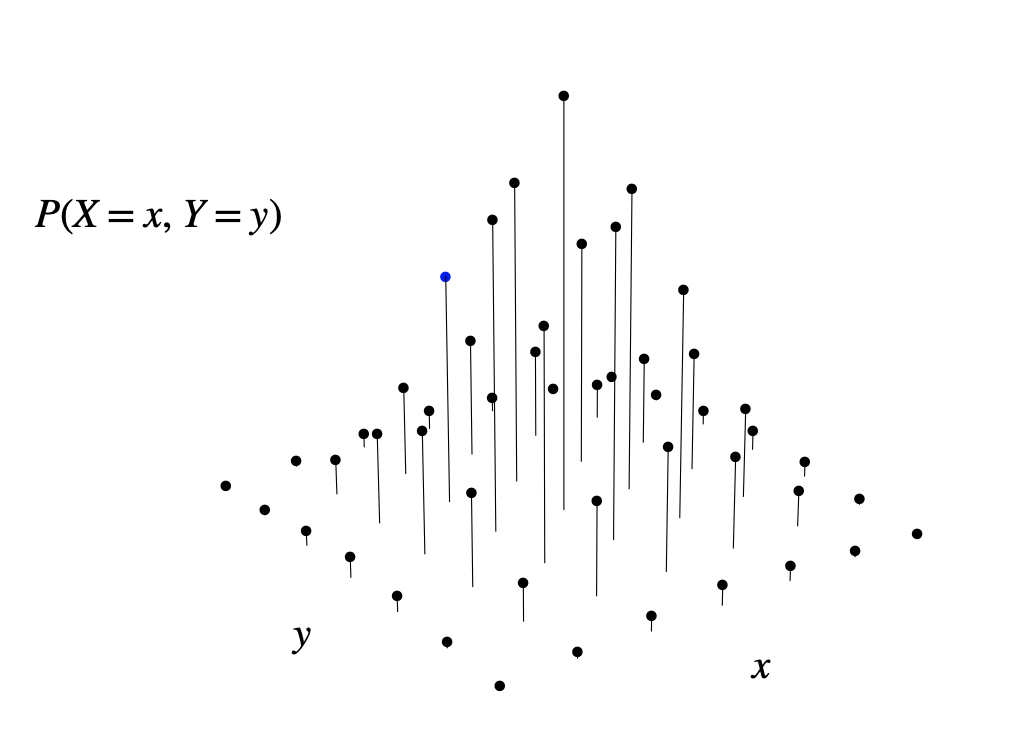
\includegraphics[width=3in]{imgs/joint_pf.png}
        \caption{Joint p.f. of discrete r.v.s $X$ and $Y$. The height of a vertical bar at 
        $(x,y)$ represents the probability $P(X=x, Y=y)$. The total summed heights of the vertical
        bars must be 1.}
    \end{figure}
    \item To be a valid joint p.f.
    \begin{itemize}
        \item The probabilities of all possible outcomes of $(X,Y)$ sum to 1. That is
        \[\sum_{\text{All } (x,y)} f(x,y) = 1\]
        \item All possible values of $(X,Y)$ have a probability greater than 0 and all other 
        values have a probability of 0. That is, if $(x,y)$ is not one of the possible values 
        of $(X,Y)$, then $f(x,y)=0$.
    \end{itemize}
    \item We can find the probability of the event $(X,Y) \in C$ for any set $C$ of points 
    (ordered pairs) in the support of $(X,Y)$ by summing over the joint p.f. over $C$
    \[P[(X,Y) \in C] = \sum_{(x,y) \in C} f(x,y)\]
\end{itemize}

\textbf{Continuous Joint Distribution}
\begin{itemize}
    \item Two r.v.s $X$ and $Y$ have a continuous joint distribution if there exists a 
    nonnegative function $f$ (joint p.d.f.) defined over the entire $xy$-plane such that for 
    every subset $C$ of the plane, 
    \[P[(X,Y) \in C] = \int_C \int f(x,y) \,dxdy\]
    if the integral exists.
\end{itemize}

\textbf{Joint Probability Density Function}
\begin{itemize}
    \item If $X$ and $Y$ are continuous r.v.s with joint c.d.f $F(x,y)$, their joint p.d.f. is 
    the derivative of the joint c.d.f. with respect to $x$ and $y$ (take the derivative of $y$
    treating $x$ as a constant, then take the derivative of $x$ treating $y$ as a constant)
    \[ f(x,y) = \frac{\partial^2}{\partial x \partial y} F(x,y) \]
    \begin{figure}[H] 
        \centering 
        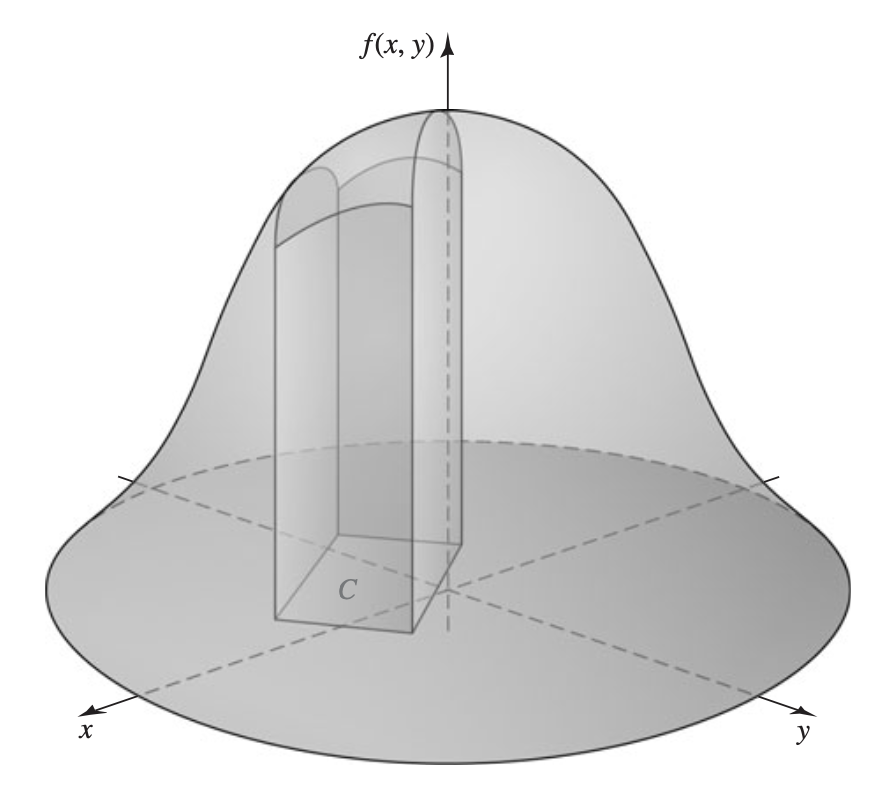
\includegraphics[width=3in]{imgs/joint_pdf.png}
        \caption{Joint p.d.f. of continuous r.v.s $X$ and $Y$. When integrating over the region 
        $C$, we are calculating the volume under the surface of the joint p.d.f and above $A$.
        The total volume under a valid joint p.d.f. is 1.}
    \end{figure}
    \item To be a valid joint p.d.f.
    \begin{itemize}
        \item The joint p.d.f. of $X$ and $Y$ must integrate to 1, that is, $\int_{-\infty}^{\infty}
        \int_{-\infty}^{\infty} f(x,y) \,dxdy =1$.
        \item For all $x$, $f(x) \ge 0$.
    \end{itemize}
\end{itemize}

\textbf{Mixed Bivariate Distributions}\
\begin{itemize}
    \item Sometimes, we must consider a mixed bivariate distribution in which we have one 
    discrete r.v. and one continuous r.v.
\end{itemize}

\textbf{Joint Probability Function/Probability Density Function}
\begin{itemize}
    \item Let $X$ and $Y$ be r.v.s such that $X$ is discrete and $Y$ is continuous. Suppose 
    that there is a function $f(x,y)$ (join p.f./p.d.f. of $X$ and $Y$) defined on the $xy$-
    plane such that, for every pair $A$ and $B$ of subsets of the real numbers,
    \[P(X \in A, Y \in B) = \int_B \sum_{x \in A} f(x,y) \,dy\]
    if the integral exists.
\end{itemize}

\textbf{Joint Cumulative Distribution Function}
\begin{itemize}
    \item The joint c.d.f. of two continuous r.v.s $X$ and $Y$ is define as the function $F$ such 
    that for all values of $x$ and $y$ $(-\infty < x < \infty, -\infty < y < \infty)$ 
    \[F(x,y)=P(X \le x, Y \le y) = \int_{-\infty}^{y} \int_{-\infty}^{x} f(r,s) \,drds\]
    \item The probability that an event occurs such that $X \le x$ and $Y \le y$.
\end{itemize}
\end{document}
